\chapter{Lecture 18 - Sturm-Liouville Problems}
\label{ch:lec18}
\section{Objectives}
\begin{itemize}
\item Define regular/singular Sturm-Liouville eigenvalue problems and give properties of their solutions.
\item Do an example problem for finding eigenvalues and eigenfunctions.
\item Do an example problem for transforming a linear, second-order, homogeneous boundary value problem into self-adjoint form.
\end{itemize}

\section{Regular Sturm-Liouville Eigenvalue Problem} \index{Sturm-Liouville Eigenvalue Problem}
We have solved several differential equations in this class.  All of the boundary value problems that we have solved so far are special cases of a more general framework called Sturm-Liouville eigenvalue problems. That is what we wish to discuss in this lecture.

For the regular Sturm-Liouville Eigenvalue problem we hope to solve:\marginnote{\textbf{Note:} for Equation \ref{eq:sturm-liouville-evp}, $r(x)$, $r^{\prime}(x)$, $q(x)$, and $p(x)$ must be real-valued and continuous on the interval $x \in (a,b)$.  Also $p(x)>0$ and $r(x)>0$ for all $x\in(a,b)$.  These are important conditions that should be verified each time you encounter a new problem.  The constant $\lambda$ is referred to as an \emph{eigenvalue}.}
\begin{equation}
\frac{d}{dx}\left[r(x)u^{\prime}\right] + \left(q(x) + \lambda p(x)\right)u = 0,  \ \ x\in(a,b)
\label{eq:sturm-liouville-evp}
\end{equation}
subject to the boundary conditions:
\begin{align*}
A_1u(a) + B_1u^{\prime}(a) &= 0, \text{ where }A_1,\text{ and }B_1\text{ are not both zero.} \\
A_2u(b) + B_2u^{\prime}(b) &= 0, \text{ where }A_2,\text{ and }B_2\text{ are not both zero.}
\end{align*}
Note that these boundary conditions are referred to as \emph{homogeneous}.  The same rule that we use to decide if a differential equation is homogeneous apply in the same way to the boundary conditions.\marginnote[-1.0cm]{For ODEs that we solved in earlier lectures, we routinely dealt with problems having non-homogeneous boundary conditions.  As we go forward to solve linear partial differential equations using separation of variables, it will be \emph{essential} that the boundary conditions are homogeneous.  So you should be sure that you know how to check/verify that condition.}  For a boundary value problem to be homogeneous, \emph{both} the differential equation \emph{and} boundary conditions must be homogeneous.

\vspace{5.0cm}

\noindent\underline{Properties of the Regular Sturm-Liouville problem:}
\begin{enumerate}
\item There exist an infinite number of real eigenvalues that can be arranged in increasing order. (e.g. $\lambda_1 < \lambda_2 < \lambda_3 < \cdots < \lambda_n < \cdots$)
\item For each eigenvalue, $\lambda_n$, there is exactly one eigenfunction, $u_n(x)$, that is a solution to the problem.

\item Eigenfunctions corresponding to different eigenvalues are linearly independent.

\item The set of eigenfunctions is orthogonal with respect to $p(x)$ on the interval $[a,b]$.  In other words: $\int_{a}^{b}u_n(x) u_m(x) p(x) \ dx = 0$ if $n \ne m$.

\item The set of eigenfunctions is complete on the interval $[a,b]$.  In other words, for any (reasonable) $f(x)$, we can represent $f(x)$ as a linear combination of those eigenfunctions: $f(x) = \sum_{n=0}^{\infty} c_n u_n(x)$.\sidenote{Another way of saying this is that no function, $f(x)$, can be orthogonal to \emph{all} of the eigenfunctions, $u_n(x)$, on the interval $[a,b]$.

To obtain values for the coefficients, $c_n$, we need only take the inner product with the corresponding eigenfunction, $u_n$.  i.e. multiply both sides by an orthogonal function and integrate.}
\end{enumerate}


\newthought{If $r(x)$ in} Equation \ref{eq:sturm-liouville-evp} is zero at either boundary, the problem is said to be a singular boundary value problem.  If $r(a) = r(b)$, with suitable boundary conditions, the problem is said to be a periodic boundary value problem.

\vspace{1.0cm}

\noindent\textbf{Example:} Find the eigenvalues and eigenfunctions of the following boundary value problem:\marginnote{Note that this problem is not presented in self-adjoint form.  Have faith that it is, indeed, a Sturm-Liouville eigenvalue problem and could be presented in self-adjoint form.  We will practice making this transformation later in the lecture.}
\begin{align*}
\text{Equation: }& & u^{\prime \prime}+\lambda u = 0,  \ \ x\in[0,1] \\
\text{BCs: }& & u(0) = 0, \ \ u(1) + u^{\prime}(1) = 0
\end{align*}
To fully analyze this problem we will have to consider three cases for $\lambda$: $\lambda < 0$, $\lambda = 0$, and $\lambda > 0$.

\vspace{0.5cm}

\noindent \underline{$\lambda = 0$:}  In this case, the differential equation reduces to:
\begin{equation*}
u^{\prime \prime} = 0
\end{equation*}
with general solution: $u(x) = c_1(x) + c_2$.  If we apply the boundary condition $u(0) = 0$, this implies that $u(0) = c_1(x) + c_2 = c_2 = 0$. So the solution is simplified to $u(x) = c_1(x)$.  The second boundary condition: $u(1) + u^{\prime}(1) = c_1(1) + c_1 = 2c_1 = 0 \Rightarrow c_1 = 0$. The only solution that satisfies the equation and boundary conditions for $\lambda = 0$ is the trivial solution $u(x) = 0$.\sidenote[][-1.5cm]{The trivial solution, $u(x)=0$ will always satisfy a homogeneous boundary value problem and, in general, is of little interest to us.  What we take from this part of the analysis is that we will rule out $\lambda=0$ since there are no \emph{interesting} solutions in that case.}

\vspace{4.5cm}

\noindent\underline{$\lambda < 0$:}  For this case we will assume $\lambda = -\alpha^2$ where $\alpha > 0$.  The differential equation reduces to:
\begin{equation*}
u^{\prime \prime} - \alpha^2u = 0
\end{equation*}
This equation has the general solution of:\marginnote[0.75cm]{Recall that these two solutions are equivalent.  We will generally use the first form on \emph{unbounded} intervals; the second form on \emph{bounded} intervals.}
\begin{align*}
u(x) &= c_1e^{-\alpha x} + c_2e^{\alpha x} \\
\text{ or: } & \\
u(x) &=c_1 \cosh{\alpha x} + c_2 \sinh{\alpha x} 
\end{align*}
Since this problem is posed on a bounded interval, we will choose the second form above.  Applying the first boundary condition gives us: $u(0) = c_1\cosh{0} + c_2\sinh{0} = c_1(1) + c_2(0) = 0 \Rightarrow c_1 = 0$.  Applying the second boundary condition to the current solution gives us: $u(1) + u^{\prime}(1) = c_2\sinh{1} + c_2\cosh{1} = 0$. \begin{marginfigure} 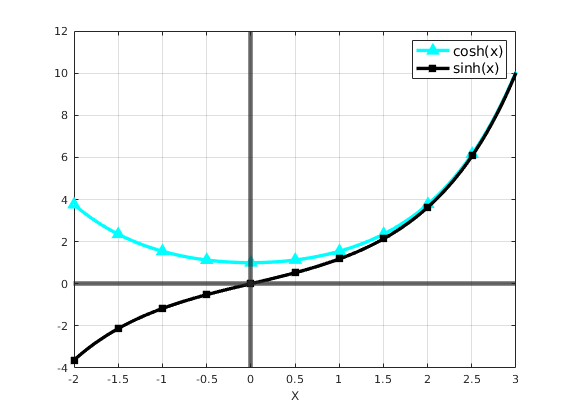
\includegraphics{cosh_and_sinh_plot.png} \end{marginfigure}  
We recall that both $\sinh{x}$ and $\cosh{x}$ are strictly positive on $x\in(0,1)$ so the only way the second boundary condition can be met is for $c_2 = 0$.  Consequently only the trivial solution, $u(x) = 0$, satisfies the governing equation and boundary conditions for the case that $\lambda < 0$.

\vspace{0.5cm}

\noindent\underline{$\lambda > 0$:} For this case we will assume $\lambda = \alpha^2$ where $\alpha > 0$.  The differential equation reduces to:
\begin{equation*}
u^{\prime \prime} + \alpha^2 u = 0
\end{equation*}
This equation has the general solution of $u(x) = c_1 \cos{\alpha x} + c_2 \sin{\alpha x}$.  Applying the first boundary condition gives us: $u(0) = c_1 \cos{0} + c_2 \sin{0} = c_1(1) + c_2(0) = 0 \Rightarrow c_1 = 0$.  Applying the second boundary condition t the current solution gives us: $u(1) + u^{\prime}(1) = c_2 \sin{\alpha} + \alpha c_2 \cos{\alpha} = 0$, or:
\begin{equation}
u(x) = c_2\left[\sin{\alpha} + \alpha \cos{\alpha}\right] = 0
\label{eq:lec18-ex1}
\end{equation}
This equation can be satisfied simply by setting $c_2 = 0$, but we will resist that temptation since that would then imply that there are \emph{no} values of $\lambda$ that admit a non-trivial solution for this problem.  Instead we will look for values of $\alpha$ such that:
\begin{equation}
\sin{\alpha} + \alpha \cos{\alpha} = 0
\label{eq:lec18-ex1-ev-eq}
\end{equation}
\begin{marginfigure}
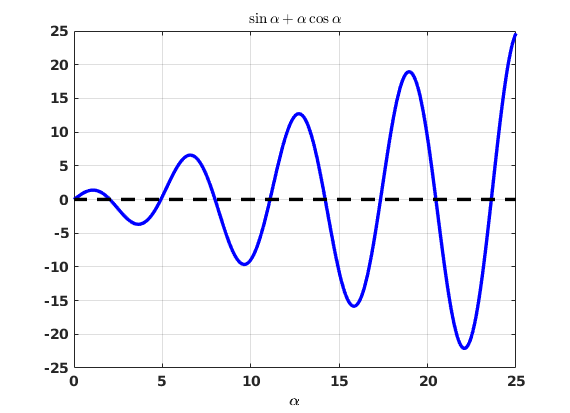
\includegraphics{lec18_evplot.png}
\caption{Plot of $\sin{\alpha} + \alpha \cos{\alpha}$.}
\label{fig:lec18-evplot}
\end{marginfigure}
We can see from Figure \ref{fig:lec18-evplot} that there are values of $\alpha$ that satisfy this condition.\sidenote{We probably should not assume as much by looking at the plot in Figure \ref{fig:lec18-evplot} but it turns out that there are infinitely many zeros.}  We will denote these eigenvalues $\alpha_1^2 = \lambda_1$, $\alpha_2^2 = \lambda_2$, $\dots$, $\alpha_n^2 = \lambda_n$ and the corresponding eigenfunctions are denoted: $u_n(x) = \sin{\alpha_n x}$.

\newthought{We will defer,} for the moment, the problem of finding the roots to Equation \ref{eq:lec18-ex1-ev-eq}. Suffice it to say that there are infinitely many distinct roots yielding the infinitely many eigenvalues to go with the infinitely many eigenfunctions. They can be found with a non-linear equation solver (``root-finder'') for which there are several reliable algorithms.

\section{Transforming Equations to Self-Adjoint Form}
Apart from sharing some theoretical tid-bits regarding Sturm-Liouville eigenvalue problems, the \emph{point} of this lecture is to highlight: a) the eigenfunctions that solve the eigenvalue problem; and b) their property of weighted orthogonality.  Recalling the last two lectures where we used an infinite set of trigonometric functions for functional expansion in a Fourier series, we will want to use \emph{other} functions for such expansions. Those other functions will be the set of eigenfunctions associated with a Sturm-Liouville eigenvalue problem.   

As previously mentioned, the eigenfunction solutions are linearly independent and orthogonal with respect to weight function $p(x)$.  We need to know what that weight function is in order to carry out an orthogonal function expansion like Fourier series.\marginnote{The sines and cosines used in Fourier series fit within this theory.  It turns out that the weight function $p(x)$ in that case is $p(x)=1$.}  

\newthought{Consider the linear,} homogeneous, second-order boundary value problem shown in Equation \ref{eq:lin-homo-bvp}:

\begin{equation}
a(x)u^{\prime \prime} + b(x)u^{\prime} + (c(x) + \lambda d(x))u = 0
\label{eq:lin-homo-bvp}
\end{equation}
where $a(x) \ne 0$ and $a(x)$, $b(x)$, $c(x)$, and $d(x)$ are continuous.  We will convert to the self-adjoint form:$\frac{d}{dx}\left[r(x)u^{\prime}\right]+[q(x)+\lambda p(x)]u =0$ by determining the functions $r(x)$, $q(x)$, and $p(x)$ as follows:
\begin{enumerate}
\item $r(x) = e^{\int \sfrac{b(x)}{a(x)} \ dx}$
\item $q(x) = \frac{c(x)}{a(x)}r(x)$
\item $p(x) = \frac{d(x)}{a(x)}r(x)$
\end{enumerate}

\vspace{5.5cm}

\noindent\textbf{Example:} Express the following equation, which has solutions $P_n(x)$ in self-adjoint form and give the orthogonality relation.\marginnote{This is Legendre's equation that we solved in a previous lecture.  $P_n(x)$ is standard notation for Legendre polynomials of order $n$.}

\begin{equation*}
\underbracket{\left(1-x^2\right)}_{a(x)}u^{\prime \prime} \underbracket{- 2x}_{b(x)}u^{\prime}+\overbracket{n(n+1)}^{\lambda}u = 0, \ \ x\in(-1,1)
\end{equation*}
From the equation, $a(x)$ and $b(x)$ are annotated; $c(x) = 0$ and $d(x) = 1$.  We first compute $r(x)$:\marginnote[0.85cm]{Here we use a $u$-substitution:
\begin{align*}
u &= \left(1-x^2\right) \\
du &= -2x \ dx 
\end{align*}
so $e^{\int \frac{-2x}{\left(1-x^2\right)} \ dx}$ = $e^{\int \frac{1}{u} \ du} $ following this substitution.
}
\begin{align*}
r(x) &= e^{\int \frac{-2x}{\left(1-x^2\right)} \ dx} \\
&= e^{\int \frac{1}{u} \ du }\\
&= e^{\ln{u}} \\
&= u \\
&= 1-x^2
\end{align*}
Now we compute $q(x):$
\begin{align*}
q(x) &= \frac{c(x)}{a(x)}r(x) \\
&= \frac{0}{\left(1-x^2\right)}\left(1-x^2\right) \\
&= 0
\end{align*}
Then $p(x)$:
\begin{align*}
p(x) &= \frac{d(x)}{a(x)} r(x) \\
&= \frac{1}{\left(1-x^2\right)}\left(1-x^2\right) \\
&= 1
\end{align*}
Therefore the boundary value problem in self-adjoint form is:
\begin{equation}
\frac{d}{dx}\left[\left(1-x^2\right)u^{\prime} \right]+\lambda_n u = 0
\end{equation}
where $\lambda_n = n(n+1)$.
As given in the problem statement, the eigenfunctions are $P_n(x)$ and the weight function $p(x) = 1$.  The orthogonality relation is:\marginnote[1.5cm]{\textbf{Note:} You will not be expected to know, by inspection, the value of $\left(P_n,P_n\right)$ but it is provided here for your information.}
\begin{equation*}
\left(P_m,P_n\right) = \int_{-1}^{1} \ P_m(x) P_n(x) (1) \ dx = 
\begin{cases}
0, & m \ne n \\
\frac{2}{2n+1}, & m = n
\end{cases}
\end{equation*}

